\chapter{Introduction}

A fundamental characteristic of sediments is whether they were deposited
in a marine or terrestrial en\-vi\-ron\-ment. This facies difference can aid reconstructing
the paleo-environment and climate or the tectonic development of sedimentary 
basins~\parencite{ding-sr-climate-2001,kempf_lower_2005,schlunegger_possible_2007,wei-2020,yang-2006}.
However, determining depositional conditions with field methods can be very difficult for
mud- and siltstones.
Traditional approaches use fossils or interpret lithostratigraphic 
observations~\parencite{nichols-sedi-2023,schlunegger-sedi-2023}, methods that are often labour-intensive
and rely on distinguishing features in the lithology. In mud- and siltstones, these can be scarce.

Salinity of modern waters is a good proxy for freshwater, brackish and marine conditions. However,
the salinity of sedimentary formation waters is difficult to measure, because it can be affected by
diagenesis~\parencite{kharaka-2003}.
Consequently, several geochemical proxies for the salinity of formation waters have been proposed.
Boron~(\acro{B}) concentrations have been studied extensively as proxies for salinity
\parencite{anovitz-grew-boron-2018, frederickson_geochemical_1960, harder-boron-1970}.
Halogens, specifically chlorine (\acro{Cl}) and bromine (\acro{Br}) 
\parencite{malcolm_behaviour_1984, Worden_1996}, trace metals like strontium (\acro{Sr}), barium (\acro{Ba}),
and gallium (\acro{Ga}) \parencite{banner-hanson-1990, bowen-sr-1956,wei-2020,ding-sr-climate-2001,yang-2006},
as well as elements related to organic content, e.g. sulphur (\acro{S}) and \TOC 
\parencite{blattmann-2019, berner-raiswell-1983}, have been applied in many contexts.

\textcite{Worden_1996} analysed existing data sets of halogen concentrations 
(\acro{Cl}, \acro{Br}, iodine (\acro{I})) in
sedimentary formation waters to reconstruct salinity. \acro{Cl}, \acro{Br} and the Cl/Br ratio
correlated with salinity, while \acro{I} was not correlated. 
Yet there was no distinct clustering of the data, preventing precise classification.

\textcite{wei-2020} reviewed a large body of work that used the trace elements
\acro{Sr}, \acro{Ba}, \acro{B}, and \acro{Ga} as proxies for salinity.
They found that particular element ratios, namely the trace elements 
\acro{B}/\acro{Ga}, \acro{Sr}/\acro{Ba}, and the indicators for primary productivity and the SO$_4$ 
concentration in the formation water \acro{S}/\acro{TOC}, 
correlated strongly with salinity. They suggest that 
combining several of those ratios improves the classification of individual samples.


\section{The Subalpine Molasse}

The \SMB
spans the area between the Jura Mountains and the Alps, extending from Geneva in the 
southwest to Lake Constance in the northeast (\cref{fig:molasse_basin}).
It has been studied extensively, first for hydrocarbons (e.g. \textcite{hartmann-oel-1919}), 
and more recently as a target for nuclear waste storage (e.g. \textcite{nagra-lager}), CO$_2$
sequestration, and geothermal energy extraction~\parencite{geomol-report}. Its overall structure,
stratigraphy and sediment composition is well established.

\subsection{Tectonic setting}

The \SMB is the foreland basin of the Alpine orogeny. It started forming during the Eocene,
driven by the northward movement and stacking of the Helvetic nappe~\parencite{weissert-stoessl-2010}. 
The basin strikes southwest-northeast across central Switzerland (\cref{fig:molasse_basin}). 
Flexure of the crystalline basement begins northwest of the folded Jura and dips southeast,
reaching a depth of approximately 6 km beneath the Alpine front (\cref{fig:molasse_profile}). 

The overthrusting of the Helvetic and Penninic nappes caused deformation of the 
sediments in the basin. \Cref{fig:molasse_profile} shows a triangular zone (\acro{BT}) of deformed
molasse beginning under the overthrust nappes, reaching the surface north of the
alpine front (\acro{AF}). That zone of deformed sediments, termed the \emph{Subalpine Molasse},
reaches the surface along the entire alpine arc (\cref{fig:molasse_basin}).

\begin{figure}
    \centering
    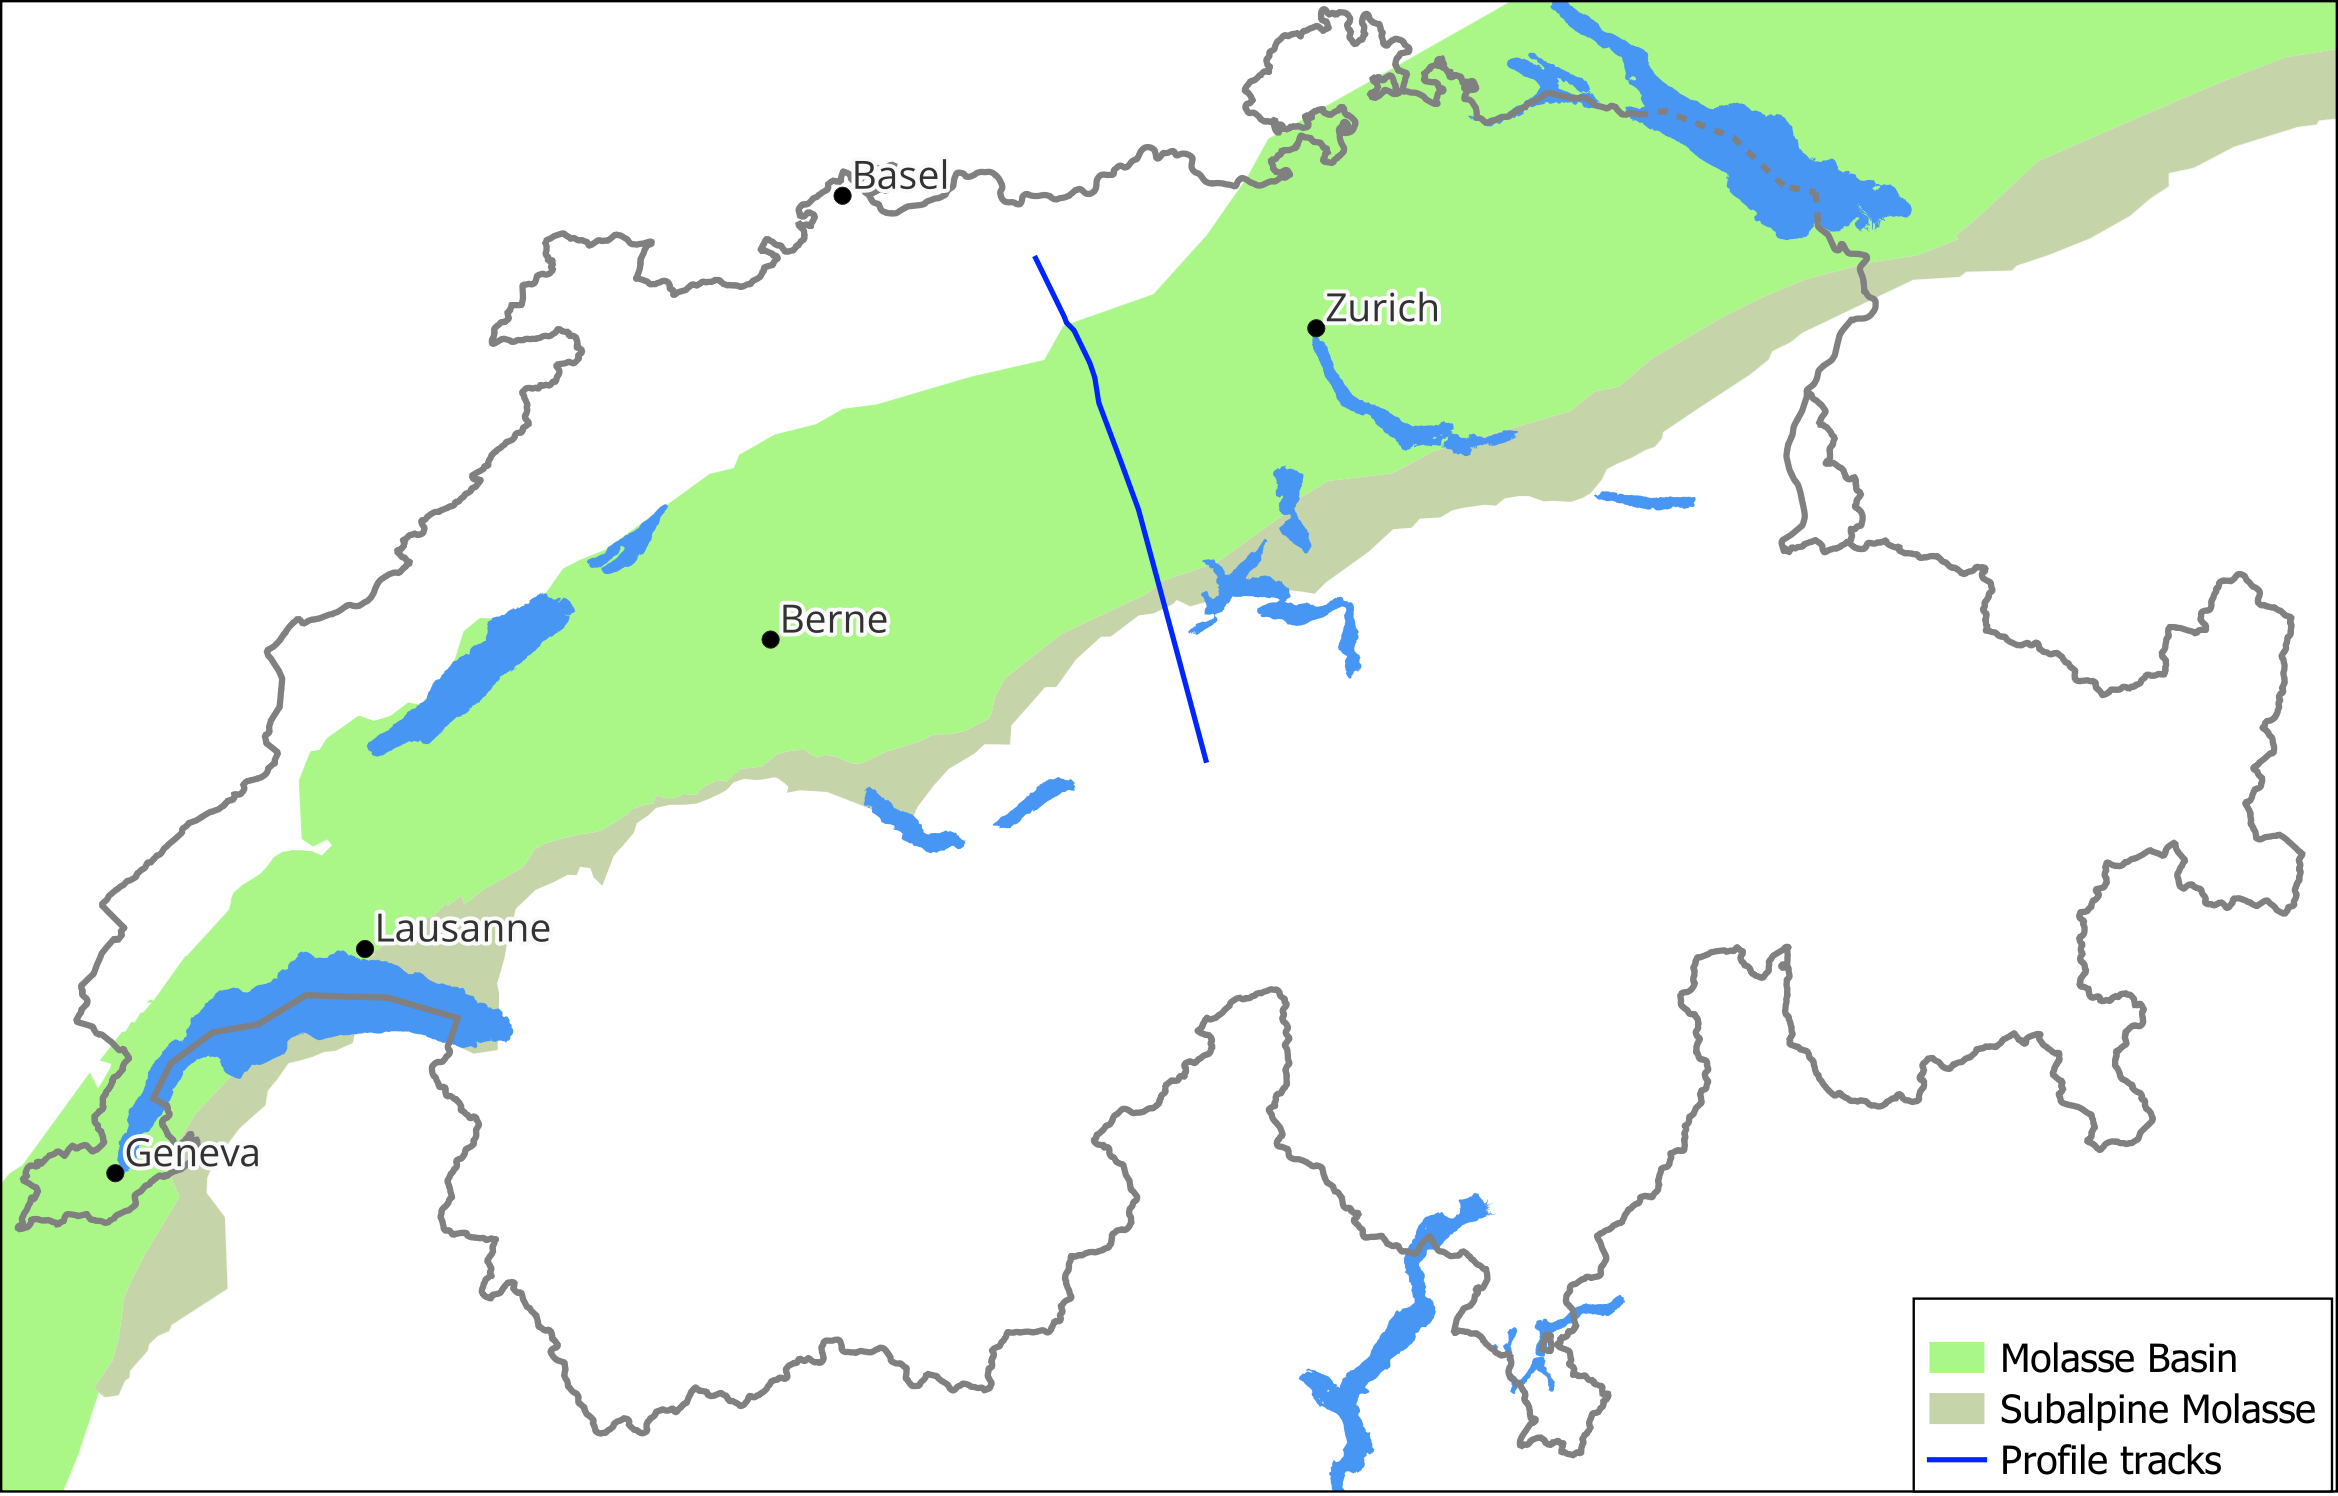
\includegraphics[width=0.8\textwidth]{img/molasse_basin.png}
    \caption{The extent of the molasse basin in Switzerland. The Subalpine Molasse is part of
    the molasse basin and forms its southern edge.}\label{fig:molasse_basin}
\end{figure}

\subsection{Geology}

The sediments filling the \SMB are the erosional debris
derived from the nearby Alps, with a thin cover of quaternary deposits. 
Grain size coarsens southward from mud/silt to gravel~\parencite{heim-geologie-bd1}. 
Because the sediments originate from individual catchments, they exhibit significant lateral variation
in clast composition and lithology,
which is particularly noticeable in the conglomerates and sandstones~\parencite{heim-geologie-bd1,Nesslau_Text,schlunegger-USM-facies-1997}.
This lateral variation complicates the interpretation and correlation of stratigraphic layers without the
broader context.

The molasse sediments are 
subdivided into units based on their prevalent depositional environment (marine vs. freshwater) and age.
This subdivision into \UMM and \USM
of Oligocene age, Upper Marine Molasse (\acro{OMM}) and \OSM
of Miocene age dates back to at least \textcite{heer-flora-1855} (\cref{fig:strati}).
The \UMM contains only mud-, silt- and sandstones, the \USM also contains pebbly conglomerates
and some freshwater carbonates~\parencite{heim-geologie-bd1}.
The subalpine molasse consists only of \UMM and \USM.
Throughout most of the basin, the molasse sediments unconformably lie on of the Mesozoic marine sediments of the 
northern Tethys \parencite{weissert-stoessl-2010}.
Along the Alpine front, the molasse stratigraphically overlays the 
flysch of the Helvetic nappe, but may also be overthrust by it. 
The reconstruction in \cref{fig:molasse_profile}
indicates that much of the subsurface structure is yet unknown.

\begin{figure}
    \centering
    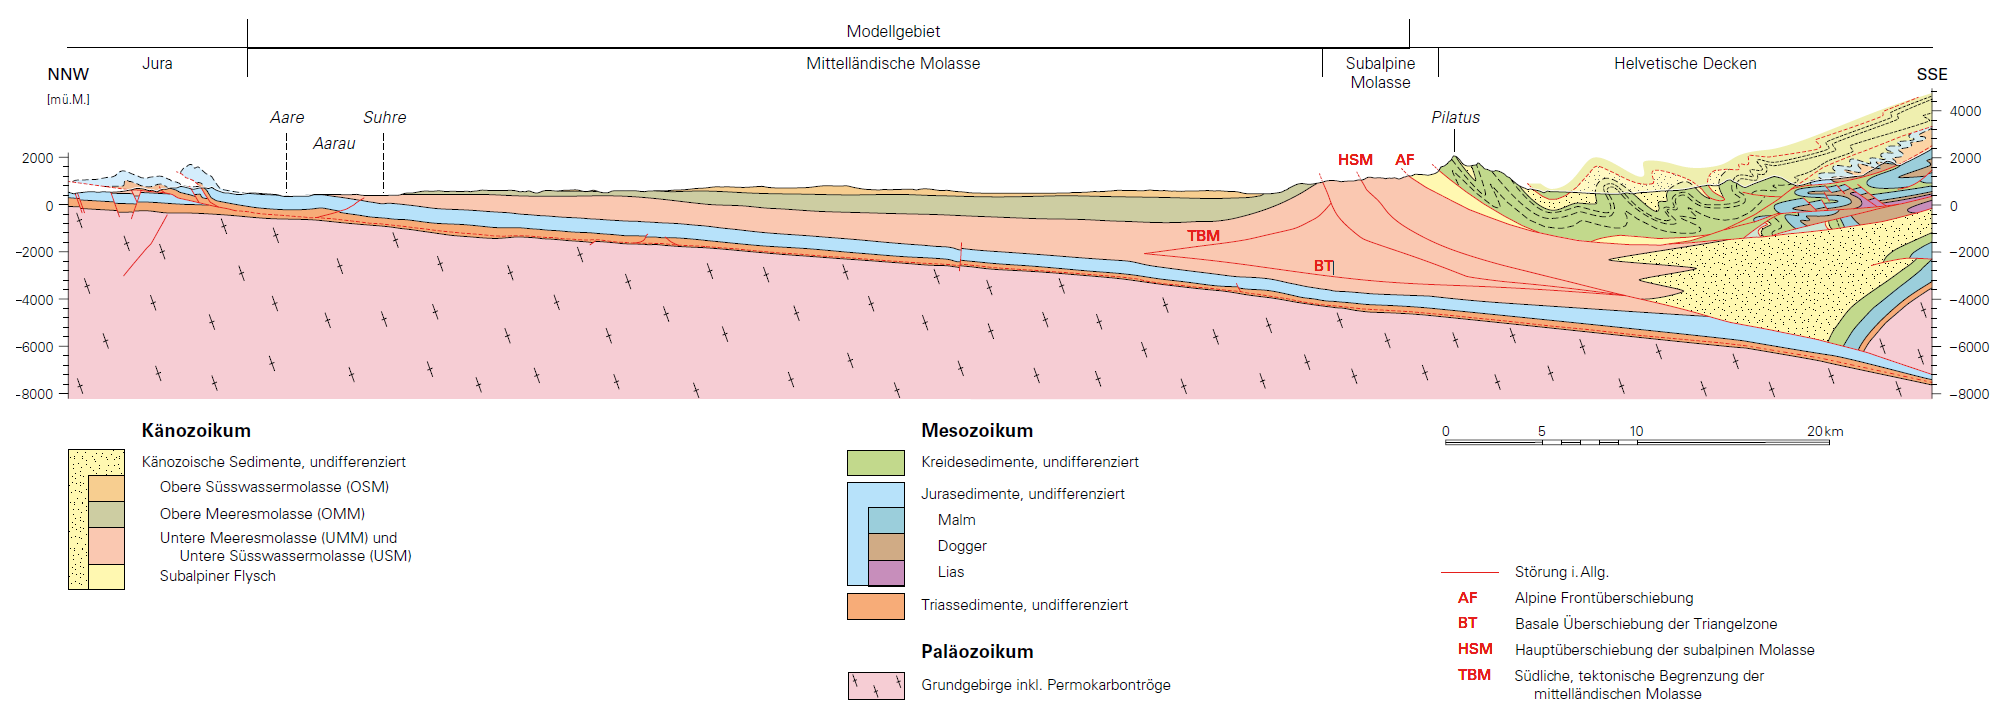
\includegraphics[width=\textwidth]{img/molasse_profile.png}
    \caption{Profile through the central SMB and bordering mountain 
    ranges~\parencite{geomol-2017}. Profile track shown in \protect\cref{fig:molasse_basin}.}\label{fig:molasse_profile}
\end{figure}

The division of \SMB units by facies is based
on macro fossils in some layers, assuming the fossil-poor surrounding
layers stem from the same depositional environment. \textcite{heim-geologie-bd1} introduced the important
qualification that the units are \emph{predominantly} (vorherrschend) of marine or freshwater
origin, rather than exclusively so. Various authors have reported such inconsistencies
between overarching unit classification and the actual depositional environment of the
sediments~\parencite{Linth_Text, Nesslau_Text}.

Determination of facies in these units is difficult, because fossils are sparse
and often not facies characteristic~\parencite{Nesslau_Text}. Additionally, many
units in the \SMB consist of mud- and siltstones, whose depositional environment
is difficult to determine using field methods alone~\parencite{Einsiedeln_Text}.
Recent works have used nanofossils to determine facies and age~\parencite{kempf_lower_2005}.

\begin{figure}
    \centering
    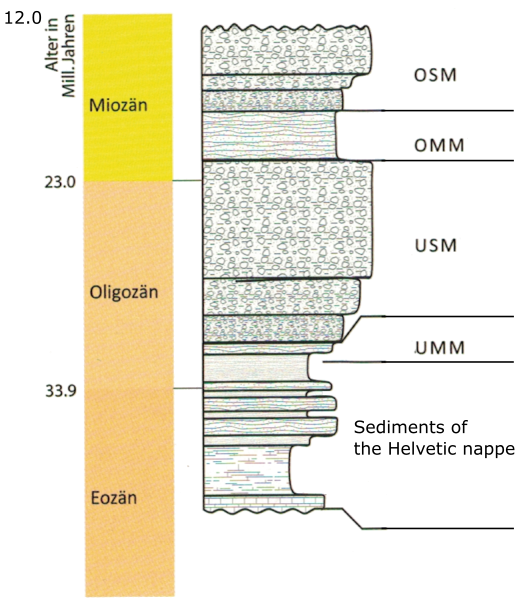
\includegraphics[width=0.3\textwidth]{img/molasse_simple_strati_mod.png}
    \caption{Stratigraphy and ages of the molasse sediments.
     Modified after \protect\textcite{weissert-stoessl-2010}.}\label{fig:strati}
\end{figure}

\section{Goals}

Advances in instrumental analyses for trace elements in rock samples,
e.g. \XRF or mass spectrometry, 
promise faster and easier access to geochemical analyses \parencite{ichikawa-xrf-2016,he_rapid_2018, he_determination_2019}.
This work investigates the utility of \XRF and \ICPMS for
measuring (trace) elements in mud- and siltstones, and the
use of previously published ratios of \acro{Sr}/\acro{Ba}, 
\acro{Cl}/\acro{Br} and \acro{S}/\acro{TOC} to characterize the
depositional environment of clay-rich sediments.
As a case study, samples from the Subalpine Molasse around Vorderthal, Switzerland are used~(\cref{fig:study_area}).

The experiments will:
\begin{itemize}
    \item Test whether \citeauthor{Worden_1996}'s \citeyear{Worden_1996} method 
    using the \acro{Cl}/\acro{Br} ratio is sufficient for a full classification.
    \item Test if the linear relationships for the \acro{Sr}/\acro{Ba}, 
    \acro{Cl}/\acro{Br} and \acro{S}/\acro{TOC} ratios determining the 
    fresh, brackish and marine
    water distinction established by \textcite{wei-2020} holds for our samples.
    \item Validate and if necessary update the geological map of the study 
    area~(\cref{fig:study_area}).
\end{itemize}

\begin{figure}[h]
\centering
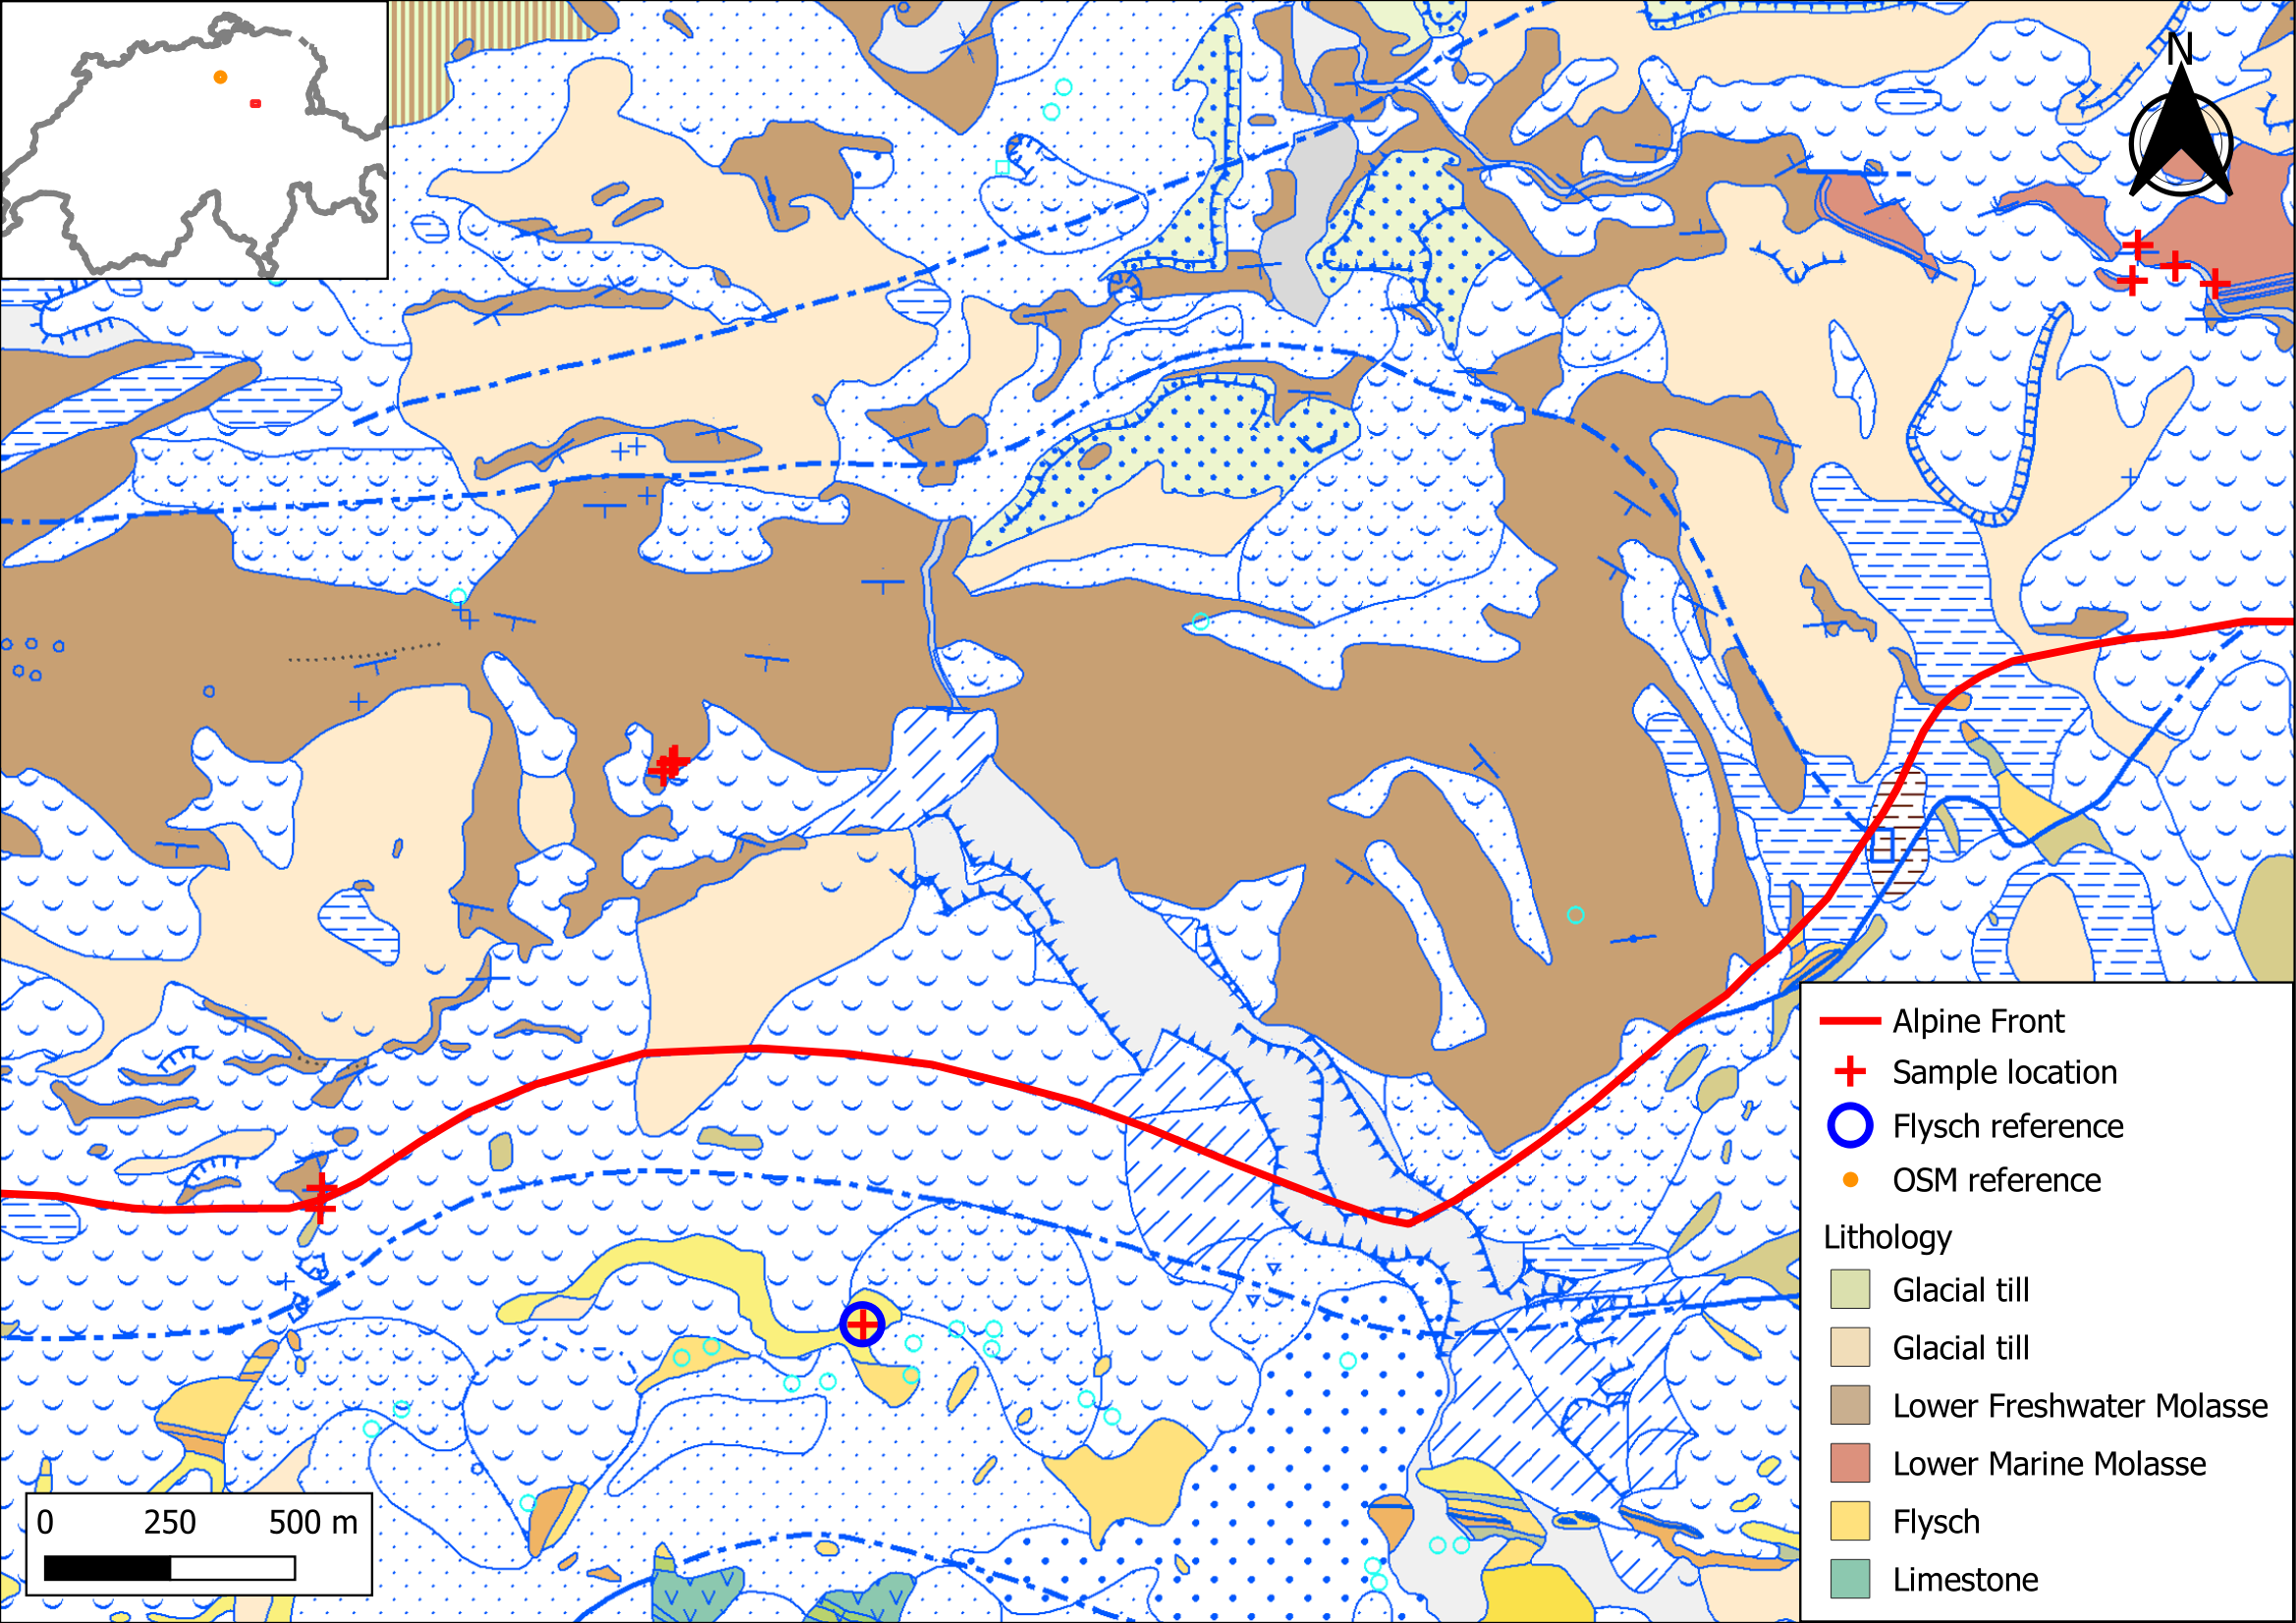
\includegraphics[width=.9\textwidth]{img/study_area.png}
\caption{The study area with sample locations. The \OSM reference location is at the orange
dot in the overview insert. Approx. GPS coordinates: 47.121420, 8.882903.
Modified from \citeauthor{swisstopo}.}\label{fig:study_area}
\end{figure}